% THIS IS SIGPROC-SP.TEX - VERSION 3.1
% WORKS WITH V3.2SP OF ACM_PROC_ARTICLE-SP.CLS
% APRIL 2009
%
% It is an example file showing how to use the 'acm_proc_article-sp.cls' V3.2SP
% LaTeX2e document class file for Conference Proceedings submissions.
% ----------------------------------------------------------------------------------------------------------------
% This .tex file (and associated .cls V3.2SP) *DOES NOT* produce:
%       1) The Permission Statement
%       2) The Conference (location) Info information
%       3) The Copyright Line with ACM data
%       4) Page numbering
% ---------------------------------------------------------------------------------------------------------------
% It is an example which *does* use the .bib file (from which the .bbl file
% is produced).
% REMEMBER HOWEVER: After having produced the .bbl file,
% and prior to final submission,
% you need to 'insert'  your .bbl file into your source .tex file so as to provide
% ONE 'self-contained' source file.
%
% Questions regarding SIGS should be sent to
% Adrienne Griscti ---> griscti@acm.org
%
% Questions/suggestions regarding the guidelines, .tex and .cls files, etc. to
% Gerald Murray ---> murray@hq.acm.org
%
% For tracking purposes - this is V3.1SP - APRIL 2009

\documentclass{acm_proc_article-sp}

\usepackage{url}
\usepackage{booktabs}

\pagenumbering{arabic}

\begin{document}

\title{Wikipedia as a Bipartite Network}
%\subtitle{[Extended Abstract]
%\titlenote{A full version of this paper is available as
%\textit{Author's Guide to Preparing ACM SIG Proceedings Using
%\LaTeX$2_\epsilon$\ and BibTeX} at
%\texttt{www.acm.org/eaddress.htm}}}
%
% You need the command \numberofauthors to handle the 'placement
% and alignment' of the authors beneath the title.
%
% For aesthetic reasons, we recommend 'three authors at a time'
% i.e. three 'name/affiliation blocks' be placed beneath the title.
%
% NOTE: You are NOT restricted in how many 'rows' of
% "name/affiliations" may appear. We just ask that you restrict
% the number of 'columns' to three.
%
% Because of the available 'opening page real-estate'
% we ask you to refrain from putting more than six authors
% (two rows with three columns) beneath the article title.
% More than six makes the first-page appear very cluttered indeed.
%
% Use the \alignauthor commands to handle the names
% and affiliations for an 'aesthetic maximum' of six authors.
% Add names, affiliations, addresses for
% the seventh etc. author(s) as the argument for the
% \additionalauthors command.
% These 'additional authors' will be output/set for you
% without further effort on your part as the last section in
% the body of your article BEFORE References or any Appendices.

\numberofauthors{3} %  in this sample file, there are a *total*
% of EIGHT authors. SIX appear on the 'first-page' (for formatting
% reasons) and the remaining two appear in the \additionalauthors section.
%
\author{
% You can go ahead and credit any number of authors here,
% e.g. one 'row of three' or two rows (consisting of one row of three
% and a second row of one, two or three).
%
% The command \alignauthor (no curly braces needed) should
% precede each author name, affiliation/snail-mail address and
% e-mail address. Additionally, tag each line of
% affiliation/address with \affaddr, and tag the
% e-mail address with \email.
%
% 1st. author
\alignauthor
Maximilian Klein\\
       \affaddr{OCLC Research}\\
       \affaddr{777 Mariners Island Blvd}\\
       \affaddr{San Mateo, CA, 94404}\\
       \email{kleinm@oclc.org}
% 2st. author
\alignauthor
Thomas Maillart\\
       \affaddr{School of Information}\\
       \affaddr{ University of California, Berkeley, 102 South Hall}\\
       \affaddr{Berkeley, CA 94720}\\
       \email{thomas.maillart@ischool.berkeley.edu}
% 3rd. author
\alignauthor
John Chuang\\
       \affaddr{School of Information}\\
       \affaddr{ University of California, Berkeley, 102 South Hall}\\
       \affaddr{Berkeley, CA 94720}\\
       \email{chuang@ischool.berkeley.edu}
}





\date{14 February 2014}
% Just remember to make sure that the TOTAL number of authors
% is the number that will appear on the first page PLUS the
% number that will appear in the \additionalauthors section.

\maketitle
\begin{abstract}
Abstract
\end{abstract}

% A category with the (minimum) three required fields
\category{H.4}{Information Systems Applications}{Miscellaneous}
%A category including the fourth, optional field follows...
\category{D.2.8}{Software Engineering}{Metrics}[complexity measures, performance measures]

\terms{to be completed}

\keywords{to be completed, if necessary} % NOT required for Proceedings

\section{Introduction}

3 elements. Literature. Question. Data. The need for a new metric.

2. We also inadvertently develop a new measure for the convtroversialness of articles, and the collaborativeness of a group of editors.

\subsection{criticism of alternative economy}
we are not really saying much about how the economy of wikipedia, i.e. inputs and outputs.
but still we can say something about the fact peer production, is indeed different from tradition economy.

but still might be useful to justify why we are using HH model, and what we expect as differences. 


\subsection{criticism of improving rankings approach}
no reliable metrics for ranking people, there is never a benchmark to say that we have a "BETTER" metric in terms of measuring quality, precisely because we use those to calibrate.

but still can say it is an effecient alternative metric, 

\subsection{issue of possible overfitting}
how do we justify the existence of alpha and beta as the parameter we calibrates

\subsection{ on HH method}
They had the origin of the method, and we use a refined technique.

\subsection{other}


3 elements. Literature. Question. Data. The need for a new metric.

1. A stream of economics research found success in predicting the fitness and ubiquity of products, by performing analysis on the bipartite graph of countries exporting products. Based on the casual observation that fitter countries produce less ubiquitous products, countries can be characterized and scored by their exports relative to the world market.

With some imagination Wikipedia, and many other online collaborative projects can be viewed as such a market. (Here we only consider English Wikipedia). We consider Wikipedia Editors to be our "countries", and Wikipedia Articles to be "products". Therefore a country producing a product is interpreted as an editor editing an article. We also inherit the assumption that the better editors will be those who edit the rarer articles, although we re-adjust that assumption in instructive ways later on. 


2. We develop a new measure for the degree of collaborativity of category.

Questions. Can this economics theory be applied, into other "economies"? Which is the other side of a Wikipedia question, which is "What are better ways to rank Wikipedia editor and articles, since the flawed Edit Counts and Article Metrics, are used as proxies"?



 

\section{Method}

\subsection{Model Description}
4. We need an intuitive way of understanding the iterative algorithm

We then applied the most general implementation of the $\mathbf{FQ}$ algorithm as developed for modelling the economy and competitiveness of countries. The $\mathbf{FQ}$ is a nonlinear generalization of the Hidalgo Hausman "Reflections Method". \cite{Caldarelli}. The algorithm has both a stochastic, iterative implementation, and an analytic solution. We demonstrate the iterative solution, to gain some intuition for the algorithm.

\begin{equation}
\begin{cases}
 w^*_c = A(\sum^{N_p}_{p=1} M_{cp}k_p^{-\alpha})k_c^{-\beta} \\
w^*_p = B(\sum^{N_c}_{c=1} M_{cp}k_c^{-\beta})k_p^{-\alpha}
\end{cases}
\end{equation}

At each iterative step we simultaneously rank editor "fitness", and article "ubiquity". In the linear model, the first iteration of "fitness" is the sum of articles to which that editor has contributed, and the "ubiquity" is the sum of editor who have contributed to that article. In the second iteration, say a user is as fit as the average the ubiquities of the of the pages edited. But this is all things being equal.

In the economic domain, the best products are those that are made by the fewest countries. Therefore in our average we want to give more weight to those best producing countries. This measure of good contributors being more important to success, is measured by alpha. A higher alpha means that a good product needs to be exported by the best countries. In Caldarelli, to correlate best with GDP rankings alpha = 1.5 Our result we find the  opposite - negative values of alpha. in the not competitive but collaborative wikipedia, where the best articles are produced by the highest number of editors


\section{Method}

1. The current investigation involved collecting historical data of edition and quality metrics, from 10 categories of articles in English Wikipedia, with focus on fine-grained edits by contributors to articles.

2. The chosen categories contain between 50 and 4000 articles, and between 50 and 5000 contributors have edited at least 100'000 times all the articles over their history. (c.f. table \ref{tab:statistics} for summary statistics on the categories). 

3. For each category, we constructed 10 accumulative snapshots, that is each starting from the first edit in the category until 10\% more of the categories total edits have occurred. \ref{fig:accumulative_snapshots}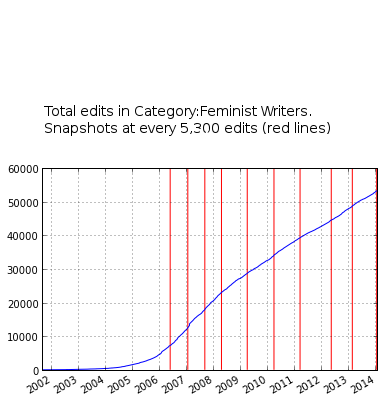
\includegraphics[scale=1]{accumulative snapshot points for Feminist Writers.png}. For each snapshot, we constructed the matrix $\mathbf{M_{e,a}}$ of contributors versus edited articles, similar to the country versus products matrix of the Economics Domain. For each snapshot, the values in $\mathbf{M_{e,a}}$ are defined as the number of edits made by editor $e$ on article $a$ in the category occurring in the snapshot time. Note that the final snapshot represents the entire history of the category up to the present date. 

\subsection{Triangular Matrices}
1. Matrix is triangular.
Perhaps not as clean as the country products matrix, but it's still triangular.

\begin{figure}[!t]
\centering
%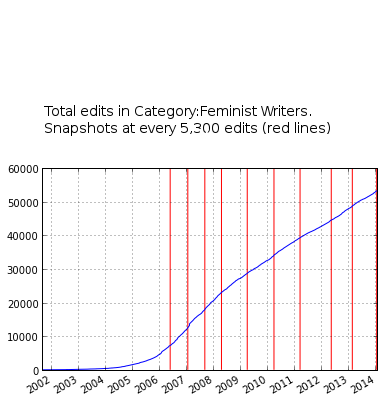
\includegraphics[width=0.9\columnwidth]{accumulative snapshot points for Feminist Writers.png}.
\caption{Triangular matrix}
\label{fig:triangle_matrix}
\end{figure}

\subsection{Interpretation of w* algorithm in the context of open collaboration}

To understand the results, we must have a firm grasp on what $\alpha$ and $\beta$ mean. They are more easily understood by roughly rewriting $\mathbf{w^*}$ as:

$$w^{*}_{e} \sim k^{1-\beta}_{e} \langle k_{a}^{-\alpha}\rangle_e $$


$$w^{*}_{a} \sim k^{1-\alpha}_{a} \langle k_{e}^{-\beta}\rangle_a $$

where $\langle k_{a}^{-\alpha}\rangle_e$ is the arithmetic average of k  $k_{a}^{-\alpha}$. 

Since we see beta and alpha are close to being additive inverses, we can just study what it means for them to increase and decrease.

For Editors.
As beta approaches one from infinity then editors are less judge by their the amount of contributions and more about the quality of the articles they contribute to. As beta becomes more negative below one, then the amount of articles is more important in predicting success.  So 'gnomier' editors are more successful in this case. So we can see beta as a style marker for a category.

The lower beta, the more a diversified editor will be successful in a Category, and the higher beta, the more a targeted quality-writing author will be successful.


\subsection{Theory of Ranking in Open Collaboration}
How this would used in an setting

\subsection{How do w* algorithm should behave in open collaboration (theory)}

It might be opposite or negative.

\subsection{Data}
1. The current investigation involved collecting historical data of edition and quality metrics, from 10 categories of articles in English Wikipedia, with focus on fine-grained edits by contributors to articles.

2. The chosen categories contain between 50 and 4000 articles, and between 50 and 5000 contributors have edited at least 100,000 times all the articles over their history. (c.f. table \ref{tab:statistics} for summary statistics on the categories). 

3. For each category, we constructed 10 accumulative snapshots, that is each starting from the first edit in the category until 10\% more of the categories total edits have occurred. \ref{fig:accumulative_snapshots}

\begin{figure}[!t]
\centering
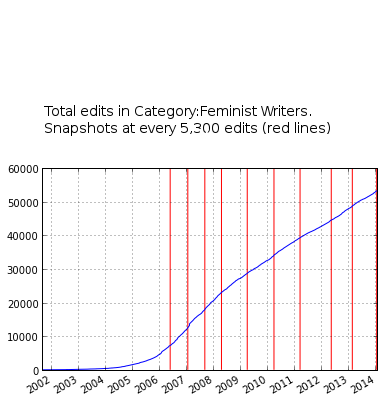
\includegraphics[width=0.9\columnwidth]{accumulative snapshot points for Feminist Writers.png}.
\caption{Cumulative snapshots, Feminist Writer}
\label{fig:cumsnaps}
\end{figure}

 For each snapshot, we constructed the matrix $\mathbf{M_{e,a}}$ of contributors versus edited articles, similar to the country versus products matrix of the Economics Domain. For each snapshot, the values in $\mathbf{M_{e,a}}$ are defined as the number of edits made by editor $e$ on article $a$ in the category occurring in the snapshot time. Note that the final snapshot represents the entire history of the category up to the present date.


 
The matrix $\mathbf{\hat{M}_{e,a}}$ is a binary representation of $\mathbf{M_{e,a}}$ where each nonzero entry is replaced with $1$. This represents if editors have touched which articles rather than how much they have touched each article. In the economics domain, the distinction of making a binary matrix out of the data is interpreted an alternative metric to GDP per capita, rather than GDP. Here we could also see the distinction as normalized editor fitness.

It has a typical triangular structure as shown on Figure \ref{fig:triangular_matrix}.

The matrix $\mathbf{\hat{M}_{e,a}}$ constitutes the basic input for implementing the Biased Markov Chain Approach, which we will call the $\mathbf{w^*}$ algorithm, which is an analytic solution to the iterative $\mathbf{W}$ algorithm. \cite{Caldarelli} 

In the iterative solution we see how certain editors start low, but then climb in rankings. This means that they are editing few articles, but those articles are of higher quality. Likewise certain articles climb over iterations, they are edited by relatively few editors, but those editors are fitter.

The output of $\mathbf{w^*}$ are a pair of rankings $ w^*_e$ and $ w^*_a$ for editors and articles respectively.

\begin{equation}
\begin{cases}
w^*_e = A(\sum^{N_a}_{a=1} M_{e,a}k_a^{-\alpha})k_e^{-\beta} \\
w^*_a = B(\sum^{N_e}_{e=1} M_{e,a}k_e^{-\beta})k_a^{-\alpha}
\end{cases}
\end{equation}

Next we collect exogenous metrics as comparison for both  $w^{*}_{e}$ and $w^{*}_{a}$, which we call  $v_e$ and $v_a$.

It is important to note that we are not competing with these metrics, but take them as state-of-the-art, Grand Truth, to which we calibrate against. We adopt a "less is more" approach. We using the exogenous variable to proxy 

Yes, indeed for authors, what we are measuring is a weaker proxy for the gnomieness.

but for artilces the exogenous metric is quite, good, i.e. similar to what we are measuring


The exogenous metric for editors $v_e$ we take is $labour hours$. For each editor the contribution history upto the snapshot point,  divide into strings of $edit sessions$, edits that occur within 1 hour of the previous edit. Then $labour hours$ are determined by subtracting the looking at the total time between the first and last edit in each edit session, and then summing the labours of each edit session. \cite{Geiger, Halfaker}. 

For an exogenous measure of article quality, $ v_a$,  we use a group of 5 text analysis metrics performed on Wikipedia articles at the lastest time in the snapshot. These are ratio of mark-up to readable text, number of headings, article length, citations per article length, and outgoing intrawiki links. To reduce the dimensionality of these 5 metrics, we perform Principal Component Analysis, and accept the principal component. Variance explained by the first principal component, was as high as .7 and never below .5 http://www-users.cs.umn.edu/~morten/publications/wikisym2013-tellmemore.pdf, http://mailer.fsu.edu/~bstvilia/papers/quantWiki.pdf \cite{ Morten}.


\subsection{Calibrating}

Having our endogenous and exegenous variables now, we perform a recursive grid search over the two dimensions of $\alpha$ and $\beta$ to find a maximum correlation between our rankings from $\mathbf{w^*}$ and our exogenous variables. Our grid search operates on the interval $[-5,5]$ with a resolution of 0.2 in on each axis. Importantly we search for negative values of $\alpha$ and $\beta$, which is not done in the Economics Domain. t

\subsection{Finding trends}

5. While the implementation presented here is strictly similar to \ref{}, the interpretation is slightly different in the context of group collaboration. Indeed, while countries competes for selling products, the hypothesis here is that Wikipedia contributors cooperate, at least in a very informal way, for improving the quality of articles.

\section{Results}

\section{Discussion}

6. {\it Refer to problems here, if any.}

\begin{table}
\centering
\caption{Summary statistics for each category}
\begin{tabular}{|c|c|l|} \hline
Non-English or Math&Frequency&Comments\\ \hline
\O & 1 in 1,000& For Swedish names\\ \hline
$\pi$ & 1 in 5& Common in math\\ \hline
\$ & 4 in 5 & Used in business\\ \hline
$\Psi^2_1$ & 1 in 40,000& Unexplained usage\\
\hline\end{tabular}
\label{tab:statistics}
\end{table}


\begin{figure}
\centering
%\epsfig{file=fly.eps}
\caption{Matrix $\mathbf{M}$ ordered by decreasing order of edits on both contributors and articles dimensions.}
\label{fig:matrix}
\end{figure}

\section{Conclusions}

%ACKNOWLEDGMENTS are optional
%\section{Acknowledgments}

%
Having our endogenous and exogenous variables now, we perform a recursive grid search over the two dimensions of $\alpha$ and $\beta$ to find a maximum correlation between our rankings from $\mathbf{w^*}$ and our exogenous variables. Our grid search operates on the interval $[-5,5]$ with a resolution of 0.2 in on each axis.


We also use a maximizing algorithm to find the values of $\alpha$ and $\beta$ which maximize the spearman $\rho$ rank correlation between our endogenous and exogenous rankings. This is performed for both of internal users ranks versus labour hours and internal article ranks and aggregated actionable article metrics.

Importantly we search for negative values of $\alpha$ and $\beta$, which is not done in the Economics Domain.

\subsection{Finding Trends over Snapshots}

The calibration technique for a category is performed at each of the ten points in the snapshot history. This allows us to track trends of $\rho$, $\alpha$, and $\beta$ over time.



5. While the implementation presented here is strictly similar to, the interpretation is slightly different in the context of group collaboration. Indeed, while countries competes for selling products, the hypothesis here is that Wikipedia contributors cooperate, at least in a very informal way, for improving the quality of articles.




\section{Results}


\subsection{high Correlations with Exogenous Variable}

THIS IS EVEN BETTER THAN HH
and by the way we have an explanation. read on to find out.

2.Once we have fitted alpha and beta we achieve high correlations with exogenous variables. We our correllation $rho$ 
 on users ranges from x to y. And on articles its better going from w, to v. These are quite high, and means that our new editor and article metrics are related to the state-of-the-art metrics that exist at the moment on Wikipedia. This gives $w^*$ a basis as an alternative metric. 
 
 Also from snapshotting we see that $rho$ increases over time, sometimes as much at 70\% from 2006 to 2014. This means that $w^*$ benefits from incorporating more contribution history.
Is this true for both articles and users?

What do we say about the fact that user correlation is worse?
-That infact editor fitness is not related to hours investment that much?
-That in the "alternative economy" we are less concerned anyway about measuring users because it all disappears in the collaborative approach to making artilces. 
 
Although $rho$ is stable and high, $\alpha$ and $\beta$ vary a lot between categories, and overtime within a category. $\alpha$ is a measure of how important it is for quality that many users edit, with lower alpha, we have a more collaborative category, where edits are more equal and egalitarean. With alpha high, the category is more being rewarding users that operate more individualistically. Beta is inversely related to alpha so the same can be said but the directions of the arguments reversed. This means we can talk of the characteristic of a category, compared to one another and compared over time. 

\subsection{Negative values of alpha and beta}
This is unexpected, and different from HH, but show anti-competitiveness. It means the contributions of less fit authors are important.

\begin{figure}[!t]
\centering
%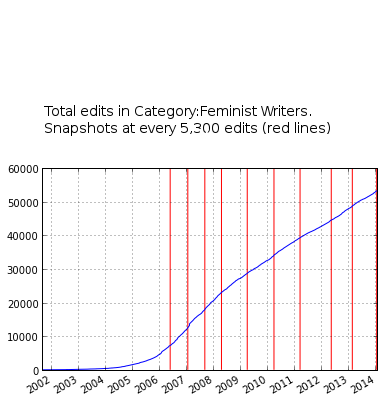
\includegraphics[width=0.9\columnwidth]{accumulative snapshot points for Feminist Writers.png}.
\caption{Landscape}
\label{fig:landscape}
\end{figure}

\subsection{Controversial Categories}
We inspeceted controversial categories. And found alphas and betas that show...

\subsection{Maybe "finding trends" subsection goes here.}
We inspect the $\rho$ maximum achievable  Spearman rank correlation between $w^*_e$ versus $v_e$ and $w^*_a$ versus $v_a$ for any values of $\alpha$ and $\beta$ over our snapshots. Behaviour of $\rho$ over time differ when considering editors, or articles. For editors, in all categories we see a trend of $\rho$ increasing over time. While the values of $\rho$ for articles are higher much higher at earlier points in the snapshots, they do not clearly increase over time, and even in some categories we see a small loss of predictive power. Since our exogenous metrics for editors and articles are different, the difference in the trend of correlation could be affected either by $w*_e$ evolving over time differently than $w*_a$, or the $v_e$ evolves over time differently than $v_a$, we did not manage to disentangle this problem.

\begin{figure}[!t]
\centering
%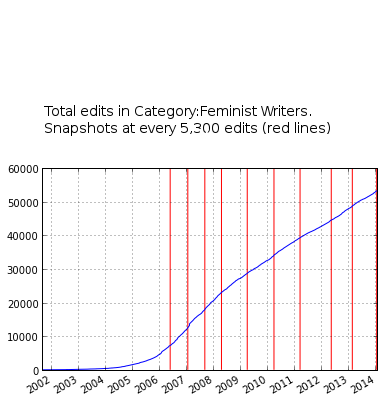
\includegraphics[width=0.9\columnwidth]{accumulative snapshot points for Feminist Writers.png}.
\caption{rtime}
\label{fig:rtime}
\end{figure}

\subsection{correlation of alpha and beta as a single paramter metric for categories}


We find that the maximizing values of $\alpha$ and $\beta$ are strongly anti-correlated. In particular for articles, the pearson correlation coefficient never drops is never below 0.8 for any category. For editors, the correlation is below 0.8 in three categories, and tend towards zero. The reduction in $\alpha$-$\beta$ anti-correlation, is itself correlated to the size of the category as determined by the number of edits, 0.65 for editors, and 0.85 for articles. 

This would mean this in that for sufficiently small categories, approximately those with less  100,000 edits, or approaximately 1,500 articles in our data, we can make the subsitituion $\alpha = - \beta$


This would mean that:

For editors
Since alpha beta are correlated 
high beta -> high gamma
low beta -> low gamma
high gamma -> best editors are less gnomie, more specialized
low gamma -> best editors are more gnomie, less specialized


For articles, as beta decreases from one and alpha increases then, the fitness of users become more important than the number of users editing. This is like, when collaboration fails because people are taking ownership. Lower alpha, and negative alpha mean more edits are more important to the success of an article.

high beta/low alpha -> high gamma
low beta/high alpha -> low gamma
high gamma -> best articles characterized by high quantity of contributor
low gamma -> best articles charachterized by high quality of contributors


Most categories fluctuate in this measure over time. Sometime there are spikes in gamma to the positive end. This would indicate??

If we look at articles in 2013 films, we do see a clear trend. Gamma starts high and ends low. That means that high quality articles shift from being edited from many people to being edited by few higher quality contributors.

It seems natural to say that $\alpha$, the importance of editor article quality, and $\beta$ the importance of editor quality would be related. For articles this would mean that they lie on a spectrum from  edited by fewer specialized editors to  many diverse editors. For editors, this would mean that editors lie on spectrum of editing many ubiquitous articles to fewer obscure articles. Let us note that this does not necessarily have to be the case. It could be that the best articles are edit both by many people and also by many specialized editors, rather than "either-or". And likewise it could be the case that  the best editors edit both many ubiquitous, and many obscure articles."

And in fact, gamma becomes less of a good assumption as the category size grows. 

Except that $\alpha , \beta$ correlation is itsself correlated to the category size.





\begin{figure}[!t]
\centering
%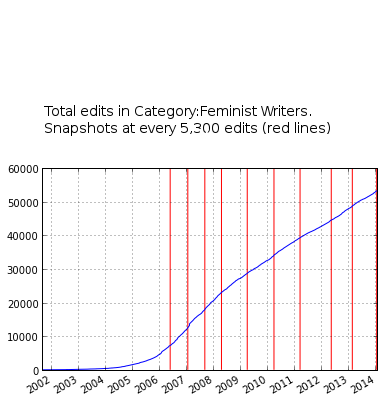
\includegraphics[width=0.9\columnwidth]{accumulative snapshot points for Feminist Writers.png}.
\caption{timeseries or maybe table}
\label{timeseries or maybe table}
\end{figure}

\subsection{Ranking Evolution}
We have three options for interpreting the evolution of ranking over time. First, what we observe is genuine to the category, that our results are specific to the categories we plot. Second, that this is a phenomena related to Wikipedia, or more generally online collaboration platforms. And third is that this an artefact of the properties of ranking. 

This paper \cite{bloom} shows that it is not inherent to ranking, so at least it is peculiar to Wikipedia. 

We have to design a small test, for instance based on hamming distance or similar, to account for the properties of ranking. 


Super Users persist over time, see the band of 




Improved correlations when remove bots. Higher correllations with binary matrices. 
Implies that edit counts are a counter productive and 


3. Highest correlations are when we have negative alpha and beta, which is about being anticompetetive. 




\section{Discussion}

A measure of controversy. Lately there have been conflicts in what categories represent.  \cite{website:nyt}

And that the super-users contribute more to sexism.\cite{website:wikinewsreporter}

 Now we have measures of importance of superuser-contributors. 


\begin{tabular}{llll}
\toprule
Category & Users & Articles &  Edits \\
\midrule
2013\_films &  5215 &     1896 &  150956 \\
American\_male\_novelists &  9946 &     2460 &  224783 \\
American\_women\_novelists &  5968 &     1936 &  138716 \\
Bicycle\_parts &   210 &       70 &    4981 \\
Computability\_theory &   272 &       92 &    7117 \\
Counterculture\_festivals &   578 &       66 &   10515 \\
Economic\_theories &  1145 &      212 &   28658 \\
Feminist\_writers &  1357 &      233 &   25738 \\
Military\_history\_of\_the\_United\_States &   854 &      180 &   20172 \\
Nobel\_Peace\_Prize\_laureates &  4165 &      104 &   91522 \\
Sexual\_acts &  2190 &       93 &   45901 \\
Yoga &   730 &      123 &   25315 \\
\bottomrule
\label{tab:statistics}
\end{tabular}

%\begin{figure}
%\caption{Matrix $\mathbf{\hat{M}}$ ordered by decreasing order of edits on both contributors and articles dimensions.}
%\label{fig:matrix}
%\end{figure}

Conclusions go here
%ACKNOWLEDGMENTS are optional
%\section{Acknowledgments}

% The following two commands are all you need in the
% initial runs of your .tex file to
% produce the bibliography for the citations in your paper.
\bibliographystyle{abbrv}

\bibliography{sigproc}  

% sigproc.bib is the name of the Bibliography in this case
% You must have a proper ".bib" file
%  and remember to run:
% latex bibtex latex latex
% to resolve all references
%
% ACM needs 'a single self-contained file'!
%
%APPENDICES are optional
%\balancecolumns
%\appendix
%Appendix A
%\section{Headings in Appendices}

\end{document}
